\subsection{Méthode des données encapsulées ou \emph{embedding}}\label{chapter-HTT_analysis-section-bg_estimation-embedding}
La méthode des données encapsulées (\emph{embedding}) permet d'estimer le bruit de fond issu du modèle standard donnant une paire de leptons tau dans l'état final en minimisant l'utilisation de simulations.
La technique, présentée en détails dans la référence~\cite{embedding}, se déroule en quatre étapes, résumées sur la figure~\ref{fig-embedding_recap} et listées ci-après:
\begin{enumerate}
\item Sélection d'une paire de muons:\\
Dans les données réelles, des paires de muons sont formées.
La paire de masse invariante la plus proche de celle du boson \Zboson\ est choisie pour la suite.
Il existe ainsi des contributions issues des processus $\Zboson\to\mu\mu$, \ttbar\ et Diboson.
\item Suppression de la paire de muons:\\
Les signaux dans le détecteur correspondant aux muons sont retirés.
Les autres signaux sont conservés pour la reconstruction de l'événement.
\item Génération d'une paire de taus:\\
Deux leptons tau sont générés.
Les propriétés cinématiques des muons initiaux sont utilisées afin d'obtenir celles des leptons tau.
Leurs valeurs exactes sont modifiées afin de rendre compte de la différence de masse entre les muons et les taus.
Plus de détails sont disponibles dans la section 5.3 de la référence~\cite{embedding}.
Les désintégrations respectives des taus en électron, muon ou tau hadronique et leurs propagations dans le détecteur sont simulées.
\item Assemblage des données sans la paire de muons et des taus générés:\\
Les traces et dépôts d'énergie des objets simulés à l'étape précédente sont ajoutés à ceux de l'événement réel, auquel les signaux associés à la paire de muons initiaux ont été retirés.
La reconstruction des événements présentée au chapitre~\refChLHCCMS\ peut alors être réalisée.
\end{enumerate}
\begin{figure}[h]
\centering
\def\EmbedPictsWidth{4}
\def\EmbedPictsMarginX{1.25}
\def\EmbedPictsMarginY{.75}
\def\EmbedPictsTxtSize{\small}
\begin{tikzpicture}
\draw (\EmbedPictsWidth/2, \EmbedPictsWidth) node [above] {\EmbedPictsTxtSize Données réelles $\Zboson\to\mu\mu$};
\node[anchor=south west,inner sep=0] at (0,0) {\frame{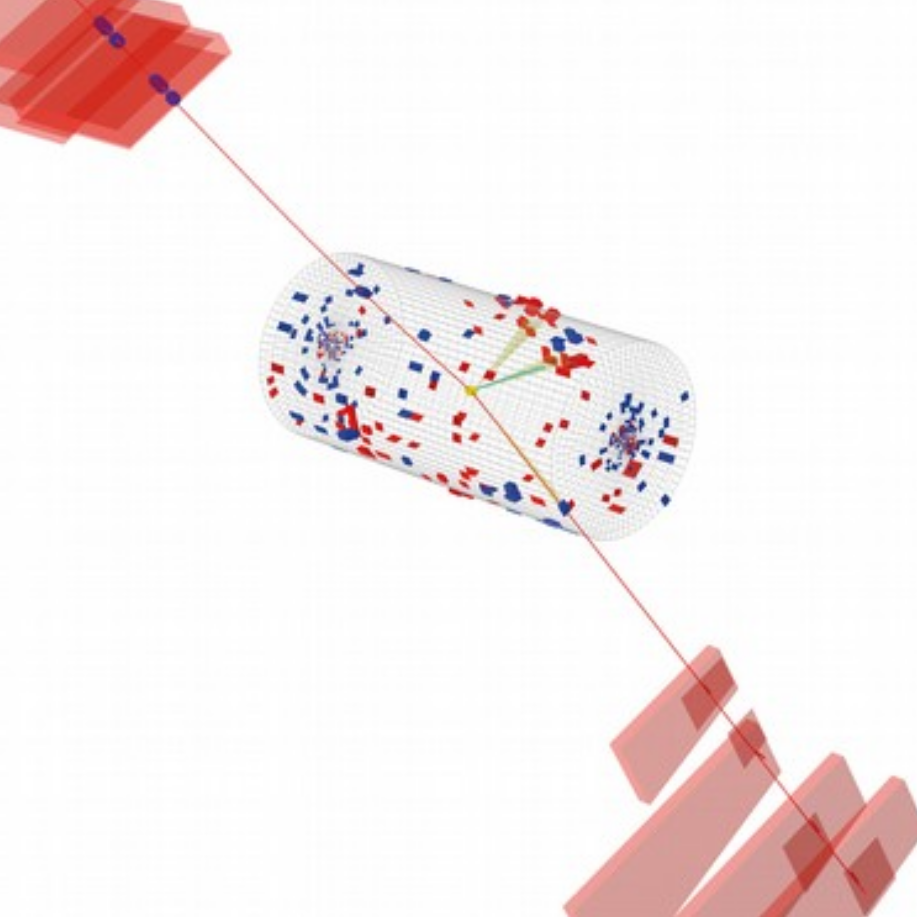
\includegraphics[width=\EmbedPictsWidth cm]{\PhDthesisdir/plots_and_images/from_embedding/Z_to_mumu_data.png}}};

\draw [-latex, very thick] (\EmbedPictsWidth+\EmbedPictsMarginX/5, \EmbedPictsWidth/2) -- + (3*\EmbedPictsMarginX/5,0);
\draw (\EmbedPictsWidth/2+\EmbedPictsWidth+\EmbedPictsMarginX, \EmbedPictsWidth) node [above] {\EmbedPictsTxtSize Supression de la paire $\mu\mu$};
\node[anchor=south west,inner sep=0] at (\EmbedPictsWidth+\EmbedPictsMarginX,0) {\frame{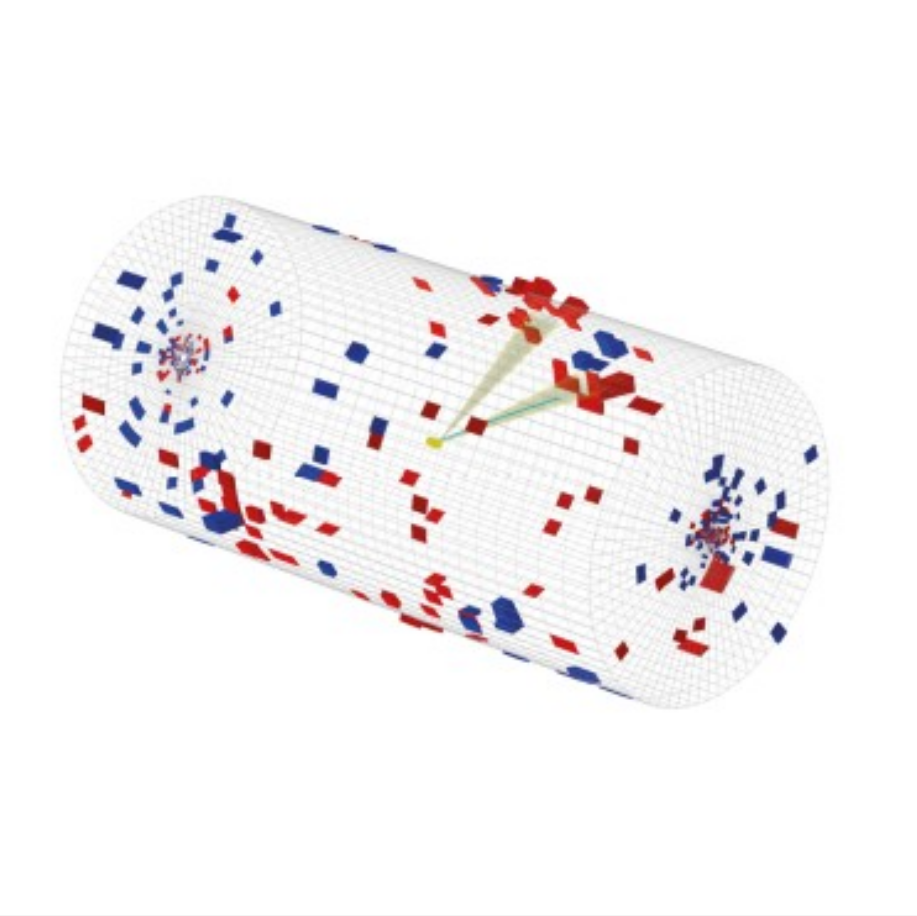
\includegraphics[width=\EmbedPictsWidth cm]{\PhDthesisdir/plots_and_images/from_embedding/remove_mumu.png}}};

\draw (\EmbedPictsWidth+\EmbedPictsMarginX,-\EmbedPictsWidth/2-\EmbedPictsMarginY) node [above left] {\EmbedPictsTxtSize Simulation des \tau};
\draw (\EmbedPictsWidth+\EmbedPictsMarginX,-\EmbedPictsWidth/2-\EmbedPictsMarginY) node [below left] {\EmbedPictsTxtSize ($\vec{p}_{\tau} \Leftrightarrow \vec{p}_{\mu}$)};
\node[anchor=south west,inner sep=0] at (\EmbedPictsWidth+\EmbedPictsMarginX,-\EmbedPictsWidth-\EmbedPictsMarginY) {\frame{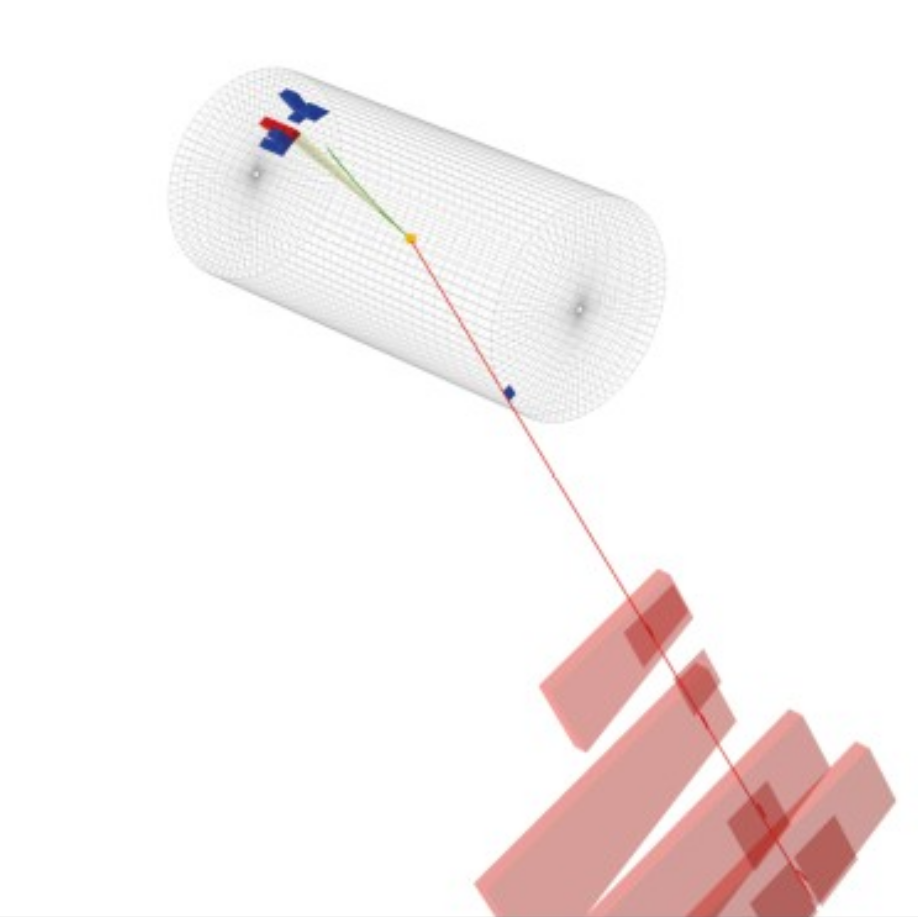
\includegraphics[width=\EmbedPictsWidth cm]{\PhDthesisdir/plots_and_images/from_embedding/Z_to_tautau_simulation.png}}};

\draw [-latex, very thick] (2*\EmbedPictsWidth+6*\EmbedPictsMarginX/5, \EmbedPictsWidth/4) -- (2*\EmbedPictsWidth+2*\EmbedPictsMarginX-\EmbedPictsMarginX/5,0);
\draw [-latex, very thick] (2*\EmbedPictsWidth+6*\EmbedPictsMarginX/5,-\EmbedPictsWidth/4-\EmbedPictsMarginY) -- (2*\EmbedPictsWidth+2*\EmbedPictsMarginX-\EmbedPictsMarginX/5,-\EmbedPictsMarginY);
\draw (2*\EmbedPictsWidth+2*\EmbedPictsMarginX+\EmbedPictsWidth/2,\EmbedPictsWidth/2-\EmbedPictsMarginY/2) node [above] {\EmbedPictsTxtSize Données encapsulées};
\node[anchor=south west,inner sep=0] at (2*\EmbedPictsWidth+2*\EmbedPictsMarginX,-\EmbedPictsWidth/2-\EmbedPictsMarginY/2) {\frame{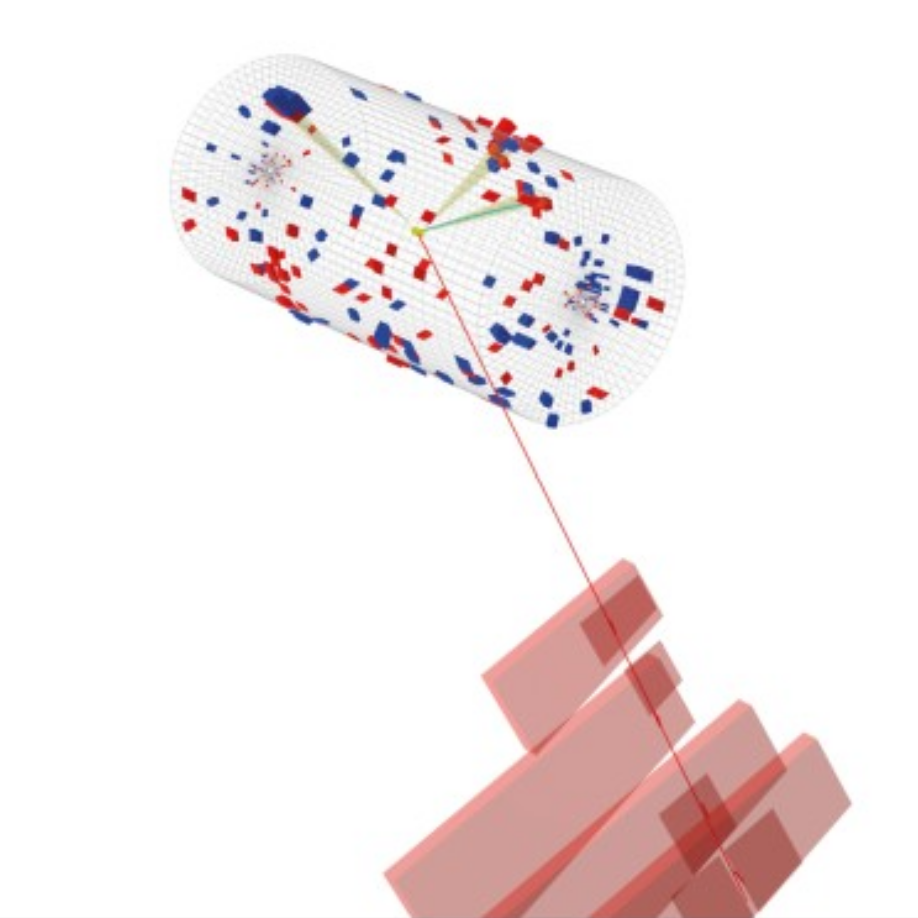
\includegraphics[width=\EmbedPictsWidth cm]{\PhDthesisdir/plots_and_images/from_embedding/embedded_event.png}}};

\clip (-1,-\EmbedPictsWidth-\EmbedPictsMarginY-.25) rectangle (3*\EmbedPictsWidth+5*\EmbedPictsMarginX/2+.25, \EmbedPictsWidth+.5);
\end{tikzpicture}
\caption[Schéma récapitulatif de la méthode des données encapsulées.]{Schéma récapitulatif de la méthode des données encapsulées~\cite{embedding}.}
\label{fig-embedding_recap}
\end{figure}
\par
Les données encapsulées nécessitent ainsi l'utilisation de simulation uniquement pour la paire de leptons taus et leurs désintégrations.
Tous les autres objets présents sont issus de données réelles.
L'amélioration de la description des données ainsi obtenue grâce à l'encapsulement est illustrée sur la figure~\ref{fig-embedding_2018mt_puppimet_illustration}, où les distributions de l'énergie transverse manquante dans les données et dans l'estimation du bruit de fond sans et avec cette méthode sont tracées.
L'accord est sensiblement amélioré pour $\MET < \SI{30}{\GeV}$.
\begin{figure}[h]
\centering

\subcaptionbox{Distribution de \MET\ sans l'encapsulement.}[.475\textwidth]
{\plotHTTcontrol{2018}{fully_classic}{mt}{puppimet}}
\hfill
\subcaptionbox{Distribution de \MET\ avec l'encapsulement.}[.475\textwidth]
{\plotHTTcontrol{2018}{emb_classic}{mt}{puppimet}}

\caption{Distributions de \MET\ pour le canal \mu\tauh\ en 2018.}
\label{fig-embedding_2018mt_puppimet_illustration}
\end{figure}
